\subsection{Einordnung im Standardmodell der Elementarteilchen}

\begin{iframe}
	\begin{figure}
		\centering
		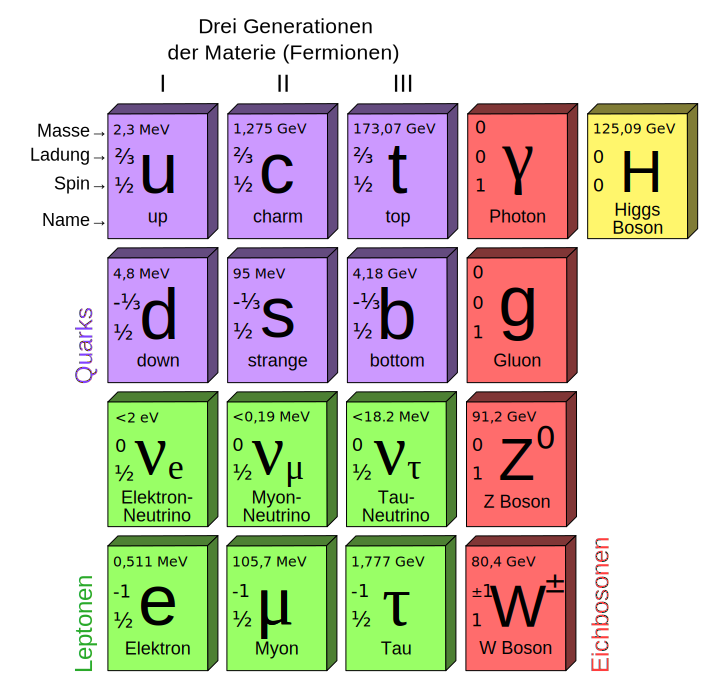
\includegraphics[width=5.5cm]{img/standardmodel}
		\caption*{Standardmodell\cite{standardmodel}}
	\end{figure}
\end{iframe}

\note[itemize]{
	\item Eichboson und Elementarteilchen
	\item schwache WW
	\item eigenes Antiteilchen
	\item W+- => elek. Teilchen WW (beta Zerfall)
	\item Z0 => auch neutral Teilchen WW (Neutrino)
}

\subsection{Elektroschwache Vereinheitlichung}
\begin{iframe}

	\begin{figure}
		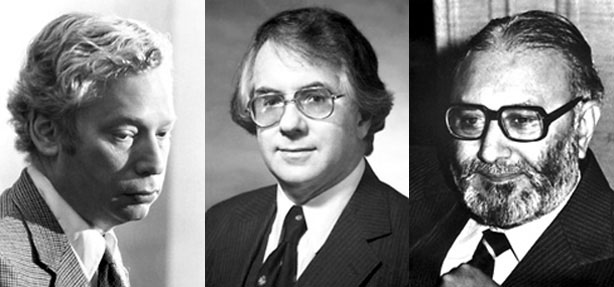
\includegraphics[width=4cm]{img/weinberg_glasgow_salam}
		\caption*{Steven Weinberg, Sheldon Glashow und Abdus Salam\cite{GSW}}
	\end{figure}
	\begin{itemize}
		\item
	\item more
	\end{itemize}
\end{iframe}

\note[itemize]{
	\item Zusammenfassung schwache + elektrom. WW %TODO date
	\item Steven Weinberg, Sheldon Glashow und Abdus Salam %TODO mehr Ort etc
	\item 1979 Nobelpreis
}

\begin{iframe}


	\framesubtitle{Austauschteilchen}
	\begin{itemize}
		\item Photon $\rightarrow$ elektromagnetische Wechselwirkung
		\pause
		\item W,Z-Boson $\rightarrow$ schwache Wechselwirkung
		\pause
		\item Gluon $\rightarrow$ starke Wechselwirkung
	\end{itemize}

\note[item]{ Kräfte durch Austauschteilchen}
\note[item] {Higgs}
\note[item] {experimentelle Bestimmung}
\end{iframe}

\begin{iframe}
	\framesubtitle{Schwacher Isospin}
	\begin{figure}
		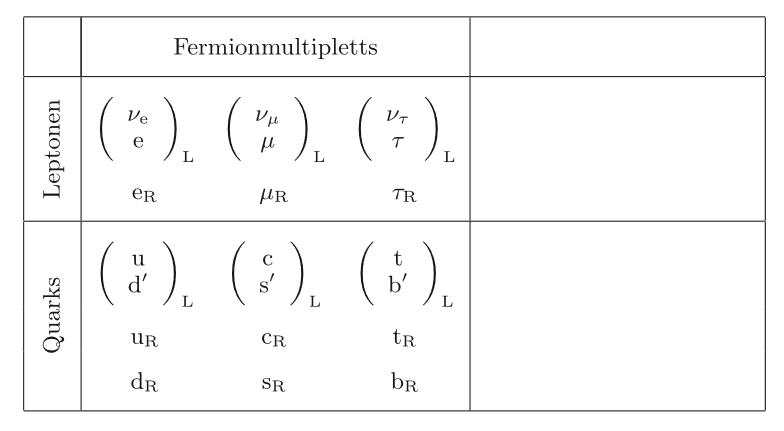
\includegraphics[height=5cm]{img/isospin1}
		\caption*{Schwacher Isospin\cite{povh}}
	\end{figure}
\end{iframe}
\newcommand{\notes}{%
\note[itemize]{
	\item Chiralität (l/r), Spinor Symmetrie
	\item analogon zu starkem Isospin
	\item Rechtshändige  Neutrinos $T_3=z=0$, keine WW, Auftreten in Natur unbekannt
}}
\notes
\begin{nframe}
	\framesubtitle{Schwacher Isospin}
	\begin{figure}
		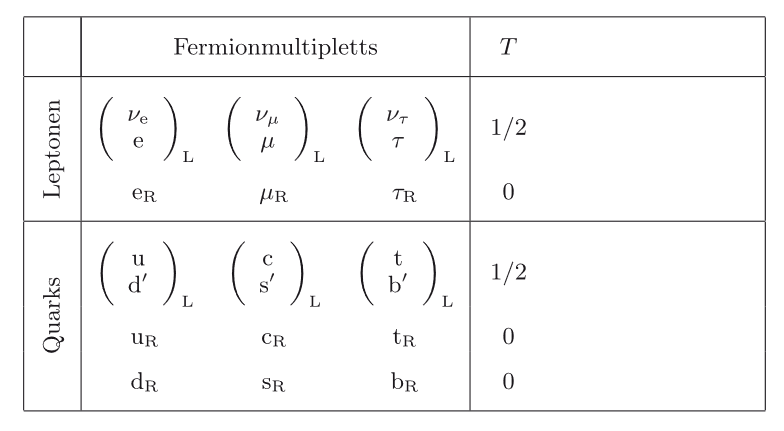
\includegraphics[height=5cm]{img/isospin2}
		\caption*{Schwacher Isospin\cite{povh}}
	\end{figure}
\end{nframe}
\notes

\begin{nframe}
	\framesubtitle{Schwacher Isospin}
	\begin{figure}
		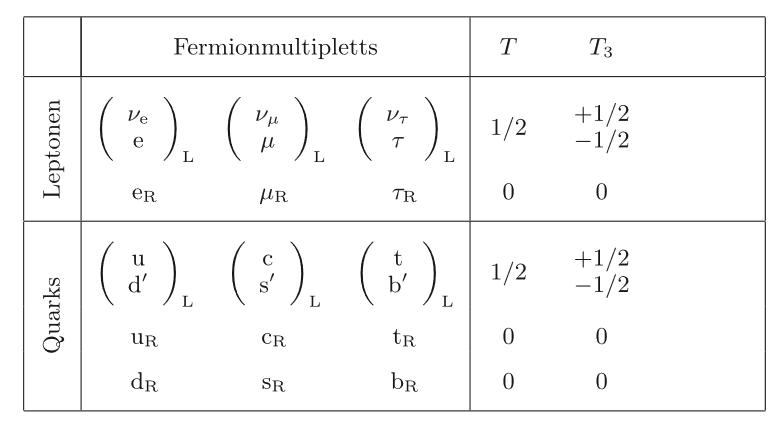
\includegraphics[height=5cm]{img/isospin3}
		\caption*{Schwacher Isospin\cite{povh}}
	\end{figure}
\end{nframe}
\notes

\begin{nframe}
	\framesubtitle{Schwacher Isospin}
	\begin{figure}
		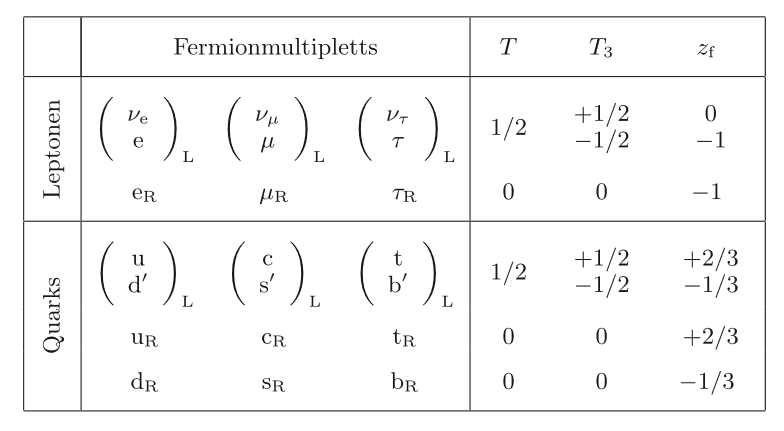
\includegraphics[height=5cm]{img/isospin}
		\caption*{Schwacher Isospin\cite{povh}}
	\end{figure}
\end{nframe}
\notes

\begin{iframe}


	\framesubtitle{Austauschteilchen}
	\begin{textblock*}{7cm}(5cm,2.5cm) % {block width} (coords)
		\begin{figure}
		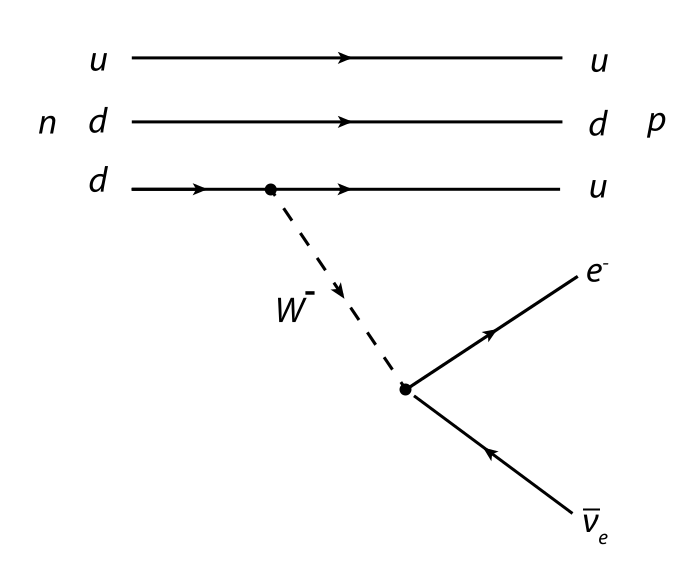
\includegraphics[height=5cm]{img/betadecay}
		\caption*{$\beta$-Zerfall\cite{beta}}
	\end{figure}
	\end{textblock*}
	\begin{itemize}
		\pause
		\item $T_3$ soll erhalten bleiben
		\pause
		\item $W^-$: $T_3=-1$
		\pause
		\item $W^+$: $T_3=1$
		\pause
		\item $W^0$: ($T=1,T_3=0$)
		\item $B^0$: ($T=0,T_3=0$)
	\end{itemize}

	\note[item]{ Bekannt aus schwacher WW }
	\note[item] {Wieso T=1}
	\note[item] {$B^0$ postuliert}
\end{iframe}

\begin{iframe}
	\begin{itemize}
	\item
		\begin{align*}
		 \ket{\gamma} &= +\cos{\theta_\text{W}} \ket{B^0} + \sin{\theta_\text{W}} \ket{W^0}	\\
		\ket{Z^0} &= -\sin{\theta_\text{W}} \ket{B^0} + \cos{\theta_\text{W}} \ket{W^0}
		\end{align*}
		\pause
	\item
		\begin{equation*}
		\cos{\theta_\text{W}}=\frac{M_\text{W}}{M_\text{Z}} \approx 0.88
		\end{equation*}
	\pause
		\item
		\begin{equation*}
		e = g \cdot sin{\theta_\text{W}}
		\end{equation*}
	\end{itemize}

	\note[item]{ Drehung um Weinberg-Winkel/elektroschwachen Mischungswinkel , Naturkonstante}
	\note[item] {orthogonal + linear Kombination}
	\note[item] {experimentelle Bestimmung}
	\note[item] {Kopplungskonstanten relevant?}
\end{iframe}

\subsection{Zerfallsbreite}
